% STATUS: ACTIVE | SSOT for the state-writing gain law with b ESTIMATED.
%   Implemented by model/controller/motion_control_law_formC_b.m and
%   test_script/integration/run_formC_b.m, both converted to this
%   parameterisation on 2026-08-18 (f7a33d0) and checked against it by an
%   identity: b_new = 1/b_old exactly, so a run locked at b_old = 9/8 must
%   reproduce one locked at b_new = 8/9, which it does to 6.1e-16.
%   x = [dw1 dw2 dw3, a_bar_w, b, m1, m2], 7 states in this writing: the two
%   MA(2) noise-memory states m1 = w_T[k-1], m2 = w_T[k-2] (production
%   ma2_aug = true, code slots 8 and 9; code slots 6-7 are inert) were added
%   2026-08-30 together with the full rank-2 Q, the estimate-throughout S8,
%   the notation line (a_o vs a_nom, f_R) and the sign of the n_w share of
%   eps_w. Verified V1-V4, ledger L42-L45. An earlier header advertised a
%   second 7-state version carrying a position-disturbance pair; it was never
%   written and the claim is withdrawn rather than left dangling. Production
%   comments referencing "S5(b)" point at it and are stale.
%         Equation-only by house convention; everything that is not an
%         equation lives in formC_state_b_ref.tex.
%         delta a does NOT appear here. Its derivation and its falsification
%         are in formC_state_dist.tex / _ref.tex, which this file does not
%         supersede and does not repeat.
% ======================================================
% Compile: xelatex formC_state_b.tex
% Path:    reference/eq17_analysis/derivation/formC_state_b.tex
% ======================================================

\documentclass[11pt,a4paper,fontset=none]{ctexart}
\usepackage[fleqn]{amsmath}
\usepackage{amssymb,bm}
\usepackage{graphicx}
\setlength{\mathindent}{0pt}
\usepackage{geometry}
\geometry{margin=2.0cm}

\setlength{\parindent}{0pt}
\setlength{\parskip}{0.80em}
\linespread{1.08}
\setlength{\abovedisplayskip}{10pt}
\setlength{\belowdisplayskip}{10pt}

\newcommand{\ba}{\bar{a}}
\newcommand{\bw}{\bar{w}}

\begin{document}

\section{Gain law}

(bars denote normalized quantities: lengths by $R$;
$a_o := \Delta t/(\gamma_N R)$ $[1/\mathrm{pN}]$ and
$a_{\mathrm{nom}} := \Delta t/\gamma_N = a_o R$ $[\mu\mathrm{m}/\mathrm{pN}]$;
$\ba := a/a_{\mathrm{nom}} = a/(a_o R) = 1/c$ for the physical gain
$a$ $[\mu\mathrm{m}/\mathrm{pN}]$;
$\bar{f} := a_o f = f/f_R$ with $f_R := \gamma_N R/\Delta t = 1/a_o$ $[\mathrm{pN}]$,
so that $\ba\,\bar{f} = \Delta\bw$;
$0 \le \ba \le 1$ on $\bw - \bw_s \ge 1/b$;
hats sit on the normalized quantities, $\hat{\ba}_w$, $\hat{b}$, $\delta\hat{\bw}$;
$e_{\theta} = \theta - \hat{\theta}$)

\begin{equation*}
\ba_{\mathrm{true}}(\bw) = 1 - \frac{9}{8\bw} + \frac{1}{2\bw^{3}}
  - \frac{57}{100\,\bw^{4}} + \frac{1}{5\bw^{5}}
  + \frac{7}{200\,\bw^{11}} - \frac{1}{25\,\bw^{12}}
\end{equation*}

\begin{equation*}
\ba'_{\mathrm{true}}(\bw) > 0 \ \ \text{on} \ \ \bw > 1
\qquad\Longrightarrow\qquad
\ba' = b_{\mathrm{true}}(\ba)\bigl(1-\ba\bigr)^{2}
\ \ \text{exactly},
\qquad
b_{\mathrm{true}} := \frac{\ba'_{\mathrm{true}}}
  {\bigl(1-\ba_{\mathrm{true}}\bigr)^{2}}
\end{equation*}

\begin{align*}
\ba_{\mathrm{true}}(1) = 0, \quad \ba'_{\mathrm{true}}(1) = 1
  &\quad\Longrightarrow\quad b_{\mathrm{true}}\bigl(\ba = 0\bigr) = 1 \\
1 - \ba_{\mathrm{true}} = \frac{9}{8\bw} + \mathcal{O}(\bw^{-3})
  &\quad\Longrightarrow\quad b_{\mathrm{true}}\bigl(\ba \to 1\bigr) = \frac{8}{9}
\end{align*}

\begin{align*}
\ba'(\ba,b) &:= b\bigl(1-\ba\bigr)^{2} \\
a_w &= a_o\,\ba_w , \qquad a_o = \frac{\Delta t}{\gamma_N R} \\
\bar{f} &= a_o f = \frac{f}{f_R}, \qquad f_R = \frac{\gamma_N R}{\Delta t} = \frac{1}{a_o}
\end{align*}

\section{Jacobians}

\begin{align*}
\frac{\partial \ba'}{\partial \ba} &= -2b\bigl(1-\ba\bigr) \\
\frac{\partial \ba'}{\partial b}   &= \bigl(1-\ba\bigr)^{2}
  = \frac{\ba'}{b}
\end{align*}

\section{True dynamics}

$\bigl(\delta\bw_j[k] := \delta\bw[k-d+j-1],\ j = 1,\dots,d+1,\ d = 2\bigr)$

\begin{align*}
\bw[k]           &= \bw_d[k] - \delta\bw_3[k] \\
\bw_d[k+1]       &= \bw_d[k] + \Delta\bw_d[k] \\
\delta\bw_1[k+1] &= \delta\bw_2[k] \\
\delta\bw_2[k+1] &= \delta\bw_3[k] \\
\delta\bw_3[k+1] &= \lambda_c\,\delta\bw_3[k] - F_{dw}[k]\,e_{\ba_w}[k]
                    - (1-\lambda_c)\bigl(m_1[k] + m_2[k]\bigr)
                    - w_T[k] + (1-\lambda_c)\,n_w[k] \\
\ba_w[k+1]       &= \ba_w[k] + \ba'_{\mathrm{true}}[k]\Bigl[
                    \Delta\bw_d[k] + (1-\lambda_c)\,\delta\bw_3[k]
                    + F_{dw}[k]\,e_{\ba_w}[k] \\
                 &\qquad\qquad\qquad
                    + (1-\lambda_c)\bigl(m_1[k] + m_2[k]\bigr)
                    + w_T[k] - (1-\lambda_c)\,n_w[k]\Bigr] \\
b[k+1]           &= b[k] \\
m_1[k+1]         &= w_T[k] \\
m_2[k+1]         &= m_1[k]
\end{align*}

\begin{align*}
F_{dw}[k] &= \bar{f}_{dw}[k] + (1-\lambda_c)\sum_{i=1}^{d}\bar{f}_{dw}[k-i] \\
w_T[k] &= \ba_w[k]\,\bar{f}_T[k] \\
\varepsilon_w[k] &= w_T[k] + (1-\lambda_c)\bigl(w_T[k-1] + w_T[k-2]\bigr)
  - (1-\lambda_c)\,n_w[k] \\
  &= w_T[k] + (1-\lambda_c)\bigl(m_1[k] + m_2[k]\bigr) - (1-\lambda_c)\,n_w[k]
\end{align*}

\section{Process model}

\begin{equation*}
\mathbf{x} = \bigl[\,\delta\bw_1,\ \delta\bw_2,\ \delta\bw_3,\ \ba_w,\ b,\ m_1,\ m_2\,\bigr]^{\top}
\qquad (d = 2;\ m_1 = w_T[k-1],\ m_2 = w_T[k-2])
\end{equation*}

\section{Estimator}

\begin{align*}
\delta\hat{\bw}_1[k+1] &= \delta\hat{\bw}_2[k] \\
\delta\hat{\bw}_2[k+1] &= \delta\hat{\bw}_3[k] \\
\delta\hat{\bw}_3[k+1] &= \lambda_c\,\delta\hat{\bw}_3[k]
  - (1-\lambda_c)\bigl(\hat{m}_1[k] + \hat{m}_2[k]\bigr) \\
\hat{\ba}_w[k+1]       &= \hat{\ba}_w[k]
  + \hat{b}[k]\bigl(1-\hat{\ba}_w[k]\bigr)^{2}
    \Bigl[\Delta\bw_d[k] + (1-\lambda_c)\,\delta\hat{\bw}_3[k]
    + (1-\lambda_c)\bigl(\hat{m}_1[k] + \hat{m}_2[k]\bigr)\Bigr] \\
\hat{b}[k+1]           &= \hat{b}[k] \\
\hat{m}_1[k+1]         &= 0 \\
\hat{m}_2[k+1]         &= \hat{m}_1[k]
\end{align*}

\section{Error dynamics}

(True $-$ Estimator; coefficients at the estimate)

\begin{align*}
e_{\delta\bw_1}[k+1] &= e_{\delta\bw_2}[k] \\
e_{\delta\bw_2}[k+1] &= e_{\delta\bw_3}[k] \\
e_{\delta\bw_3}[k+1] &= \lambda_c\,e_{\delta\bw_3}[k]
  - F_{dw}[k]\,e_{\ba_w}[k]
  - (1-\lambda_c)\bigl(e_{m_1}[k] + e_{m_2}[k]\bigr)
  - w_T[k] + (1-\lambda_c)\,n_w[k] \\
e_{\ba_w}[k+1] &= \Bigl[\,1
  + \hat{b}\bigl(1-\hat{\ba}_w\bigr)^{2}F_{dw}
  - 2\hat{b}\bigl(1-\hat{\ba}_w\bigr)
    \bigl(\Delta\bw_d + (1-\lambda_c)\delta\hat{\bw}_3
      + (1-\lambda_c)(\hat{m}_1 + \hat{m}_2)\bigr)\Bigr] e_{\ba_w}[k] \\
  &\qquad + (1-\lambda_c)\,\hat{b}\bigl(1-\hat{\ba}_w\bigr)^{2}
      \bigl(e_{\delta\bw_3}[k] + e_{m_1}[k] + e_{m_2}[k]\bigr) \\
  &\qquad + \bigl(1-\hat{\ba}_w\bigr)^{2}
      \bigl(\Delta\bw_d + (1-\lambda_c)\delta\hat{\bw}_3
      + (1-\lambda_c)(\hat{m}_1 + \hat{m}_2)\bigr) e_b[k] \\
  &\qquad + \hat{b}\bigl(1-\hat{\ba}_w\bigr)^{2}
      \bigl(w_T[k] - (1-\lambda_c)\,n_w[k]\bigr) \\
e_b[k+1] &= e_b[k] \\
e_{m_1}[k+1] &= w_T[k] \\
e_{m_2}[k+1] &= e_{m_1}[k]
\end{align*}

\begin{equation*}
\scriptsize
\setlength{\arraycolsep}{2.5pt}
\hspace*{-0.9cm}
F_e[k] =
\begin{bmatrix}
0 & 1 & 0 & 0 & 0 & 0 & 0 \\[0.4em]
0 & 0 & 1 & 0 & 0 & 0 & 0 \\[0.4em]
0 & 0 & \lambda_c & -F_{dw} & 0 & -(1-\lambda_c) & -(1-\lambda_c) \\[0.8em]
0 & 0 & (1-\lambda_c)\,\hat{b}\bigl(1-\hat{\ba}_w\bigr)^{2}
  & \begin{array}{@{}l@{}}
      1 + \hat{b}\bigl(1-\hat{\ba}_w\bigr)^{2}F_{dw} \\[0.5em]
      \quad - 2\hat{b}\bigl(1-\hat{\ba}_w\bigr)
        \bigl(\Delta\bw_d + (1-\lambda_c)\,\delta\hat{\bw}_3 \\[0.3em]
      \qquad + (1-\lambda_c)(\hat{m}_1 + \hat{m}_2)\bigr)
    \end{array}
  & \begin{array}{@{}l@{}}
      \bigl(1-\hat{\ba}_w\bigr)^{2} \\[0.5em]
      \quad \times \bigl(\Delta\bw_d + (1-\lambda_c)\,\delta\hat{\bw}_3 \\[0.3em]
      \qquad + (1-\lambda_c)(\hat{m}_1 + \hat{m}_2)\bigr)
    \end{array}
  & (1-\lambda_c)\,\hat{b}\bigl(1-\hat{\ba}_w\bigr)^{2}
  & (1-\lambda_c)\,\hat{b}\bigl(1-\hat{\ba}_w\bigr)^{2} \\[2.2em]
0 & 0 & 0 & 0 & 1 & 0 & 0 \\[0.4em]
0 & 0 & 0 & 0 & 0 & 0 & 0 \\[0.4em]
0 & 0 & 0 & 0 & 0 & 1 & 0
\end{bmatrix}
\end{equation*}

\begin{equation*}
\mathbf{q}[k] = w_T[k]\,\Bigl[\,0,\ 0,\ -1,\
\hat{b}\bigl(1-\hat{\ba}_w\bigr)^{2},\ 0,\ 1,\ 0\,\Bigr]^{\top}
 - (1-\lambda_c)\,n_w[k]\,\Bigl[\,0,\ 0,\ -1,\
\hat{b}\bigl(1-\hat{\ba}_w\bigr)^{2},\ 0,\ 0,\ 0\,\Bigr]^{\top}
\end{equation*}

\section{Measurement and innovation}

\begin{align*}
\nabla_d\bw_d[k] &= \bw_d[k] - \bw_d[k-d] \\
y_1[k] &= \delta\bw_1[k] + n_w[k] \\
y_2[k] &= \ba_w[k-d] + n_a[k]
\end{align*}

\begin{equation*}
\ba_w[k-d] = \ba_w[k]
  - b\bigl(1-\ba_w[k]\bigr)^{2}\nabla_d\bw_d[k]
\end{equation*}

\begin{align*}
\frac{\partial y_2}{\partial \ba_w}
  &= 1 + 2\hat{b}\bigl(1-\hat{\ba}_w\bigr)\nabla_d\bw_d \\
\frac{\partial y_2}{\partial b}
  &= -\bigl(1-\hat{\ba}_w\bigr)^{2}\nabla_d\bw_d
\end{align*}

\begin{equation*}
H[k] =
\begin{bmatrix}
1 & 0 & 0 & 0 & 0 & 0 & 0 \\
0 & 0 & 0 & 1 + 2\hat{b}(1-\hat{\ba}_w)\nabla_d\bw_d
  & -(1-\hat{\ba}_w)^{2}\nabla_d\bw_d & 0 & 0
\end{bmatrix}
\end{equation*}

\begin{equation*}
L[k] = P^f H^{\top}\bigl(HP^fH^{\top}+R\bigr)^{-1}
\end{equation*}

\begin{align*}
e_{y_1}[k] &= e_{\delta\bw_1}[k] + n_w[k] \\
e_{y_2}[k] &= \Bigl[1 + 2\hat{b}\bigl(1-\hat{\ba}_w\bigr)
    \nabla_d\bw_d\Bigr] e_{\ba_w}[k]
  - \bigl(1-\hat{\ba}_w\bigr)^{2}\nabla_d\bw_d\;e_b[k]
  + n_a[k]
\end{align*}

\section{Process and measurement noise}

\begin{align*}
\gamma(\bw) &= \gamma_N c(\bw) \\
\sigma^{2}_{\bar{f}_T} &= a_o^{2}\,\frac{4k_BT\gamma(\bw)}{\Delta t} \\
\kappa_T &:= \frac{4k_BT\,a_o}{R} = \frac{4k_BT\,a_{\mathrm{nom}}}{R^{2}} \\
\sigma^{2}_{w_T}[k] &= \mathrm{Var}\bigl(\ba_w[k]\,\bar{f}_T[k]\bigr)
  = \kappa_T\,\ba_w[k] \ \to\ \kappa_T\,\hat{\ba}_w[k] \\
\sigma^{2}_{n_w} &= \frac{\sigma^{2}_{n}}{R^{2}}
\end{align*}

\begin{align*}
\mathbf{g}_T &= \bigl[\,0,\ 0,\ -1,\ \hat{b}(1-\hat{\ba}_w)^{2},\ 0,\ 1,\ 0\,\bigr]^{\top} \\
\mathbf{g}_n &= (1-\lambda_c)\bigl[\,0,\ 0,\ -1,\ \hat{b}(1-\hat{\ba}_w)^{2},\ 0,\ 0,\ 0\,\bigr]^{\top} \\
Q[k] &= \kappa_T\,\hat{\ba}_w[k]\;\mathbf{g}_T\mathbf{g}_T^{\top}
  + \sigma^{2}_{n_w}\;\mathbf{g}_n\mathbf{g}_n^{\top}
\end{align*}

\begin{align*}
Q_{33} &= \kappa_T\,\hat{\ba}_w + (1-\lambda_c)^{2}\sigma^{2}_{n_w} \\
Q_{34} = Q_{43} &= -\hat{b}\bigl(1-\hat{\ba}_w\bigr)^{2}Q_{33} \\
Q_{44} &= \hat{b}^{2}\bigl(1-\hat{\ba}_w\bigr)^{4}Q_{33} \\
Q_{36} = Q_{63} &= -\kappa_T\,\hat{\ba}_w \\
Q_{46} = Q_{64} &= \hat{b}\bigl(1-\hat{\ba}_w\bigr)^{2}\kappa_T\,\hat{\ba}_w \\
Q_{66} &= \kappa_T\,\hat{\ba}_w \\
Q_{55} &= 0
\end{align*}

(white-container arm, \texttt{ma2\_aug = false}: no $m_1, m_2$, and the whole
$\mathrm{Var}(\varepsilon_w)$ sits in $Q_{33}$)
\begin{align*}
\mathrm{Var}(\varepsilon_w)[k] &= \kappa_T\Bigl(\hat{\ba}_w[k]
  + (1-\lambda_c)^{2}\bigl(\hat{\ba}_w[k-1] + \hat{\ba}_w[k-2]\bigr)\Bigr)
  + (1-\lambda_c)^{2}\sigma^{2}_{n_w}
\end{align*}

\begin{align*}
R &= \mathrm{diag}(R_1, R_2) \\
R_1 &= \sigma^{2}_{n_w} \\
R_2 &= K_{\mathrm{var}} IF_{\mathrm{var}}\bigl(\hat{\ba}_w+\xi\bigr)^{2} + d\,Q_{44} \\
K_{\mathrm{var}} &= \frac{2a_{\mathrm{cov}}}{2-a_{\mathrm{cov}}} \\
\sigma^{2}_{\delta\bw_r} &= C_{dpmr}\,\kappa_T\bigl(\hat{\ba}_w+\xi\bigr) \\
\xi &= \frac{C_n\,\sigma^{2}_{n_w}}{C_{dpmr}\,\kappa_T}
\end{align*}

\section*{Seed and prior}

\begin{align*}
\ba(\bw) &= 1 - \frac{1}{b\,(\bw-\bw_s)} \\
\frac{\partial \ba}{\partial b}\bigg|_{\bw}
  &= \frac{1}{b^{2}(\bw-\bw_s)} = \frac{1-\ba}{b} \\
\frac{\partial \ba}{\partial \bw_s}\bigg|_{\bw} &= -\,\ba'
\end{align*}

\begin{align*}
\hat{b}[0] &= b_{\mathrm{true}}\bigl(\ba \to 1\bigr) = \tfrac{8}{9} \\
P_{55}[0] = P_{bb} &= \Bigl[\sup_{\bw\in\mathcal{E}}
  \bigl|\,b_{\mathrm{true}}(\bw) - \tfrac{8}{9}\,\bigr|\Bigr]^{2} \\
\hat{\ba}_w[0] &= 1 - \frac{1}{\hat{b}[0]\,(\bw[0]-\hat{\bw}_s)}
\end{align*}

\begin{align*}
P_{44}[0] &= \bigl(\hat{\ba}'[0]\bigr)^{2}P_{\bw_s}
  + \left(\frac{1-\hat{\ba}_w[0]}{\hat{b}[0]}\right)^{2}P_{bb}
  + \mathrm{floor}_a^{2} \\
P_{45}[0] &= \frac{1-\hat{\ba}_w[0]}{\hat{b}[0]}\,P_{bb} \\
P_{\{1,2,3,6,7\}}[0] &= \mathrm{DARE}\Bigl(F_e^{\{1,2,3,6,7\}}[0],\ H_1^{\{1,2,3,6,7\}},\
  Q^{\{1,2,3,6,7\}}[0],\ R_1\Bigr)
\end{align*}

\begin{align*}
e_{\ba}(\bw)\big|_{\bw_s} &= -\,\ba'(\bw)\,e_{\bw_s}
  \ \propto\ \frac{1}{b\,(\bw-\bw_s)^{2}} \\
e_{\ba}(\bw)\big|_{b}     &= \frac{e_b}{b^{2}(\bw-\bw_s)}
\end{align*}



\clearpage

\begin{figure}[htbp]
\centering
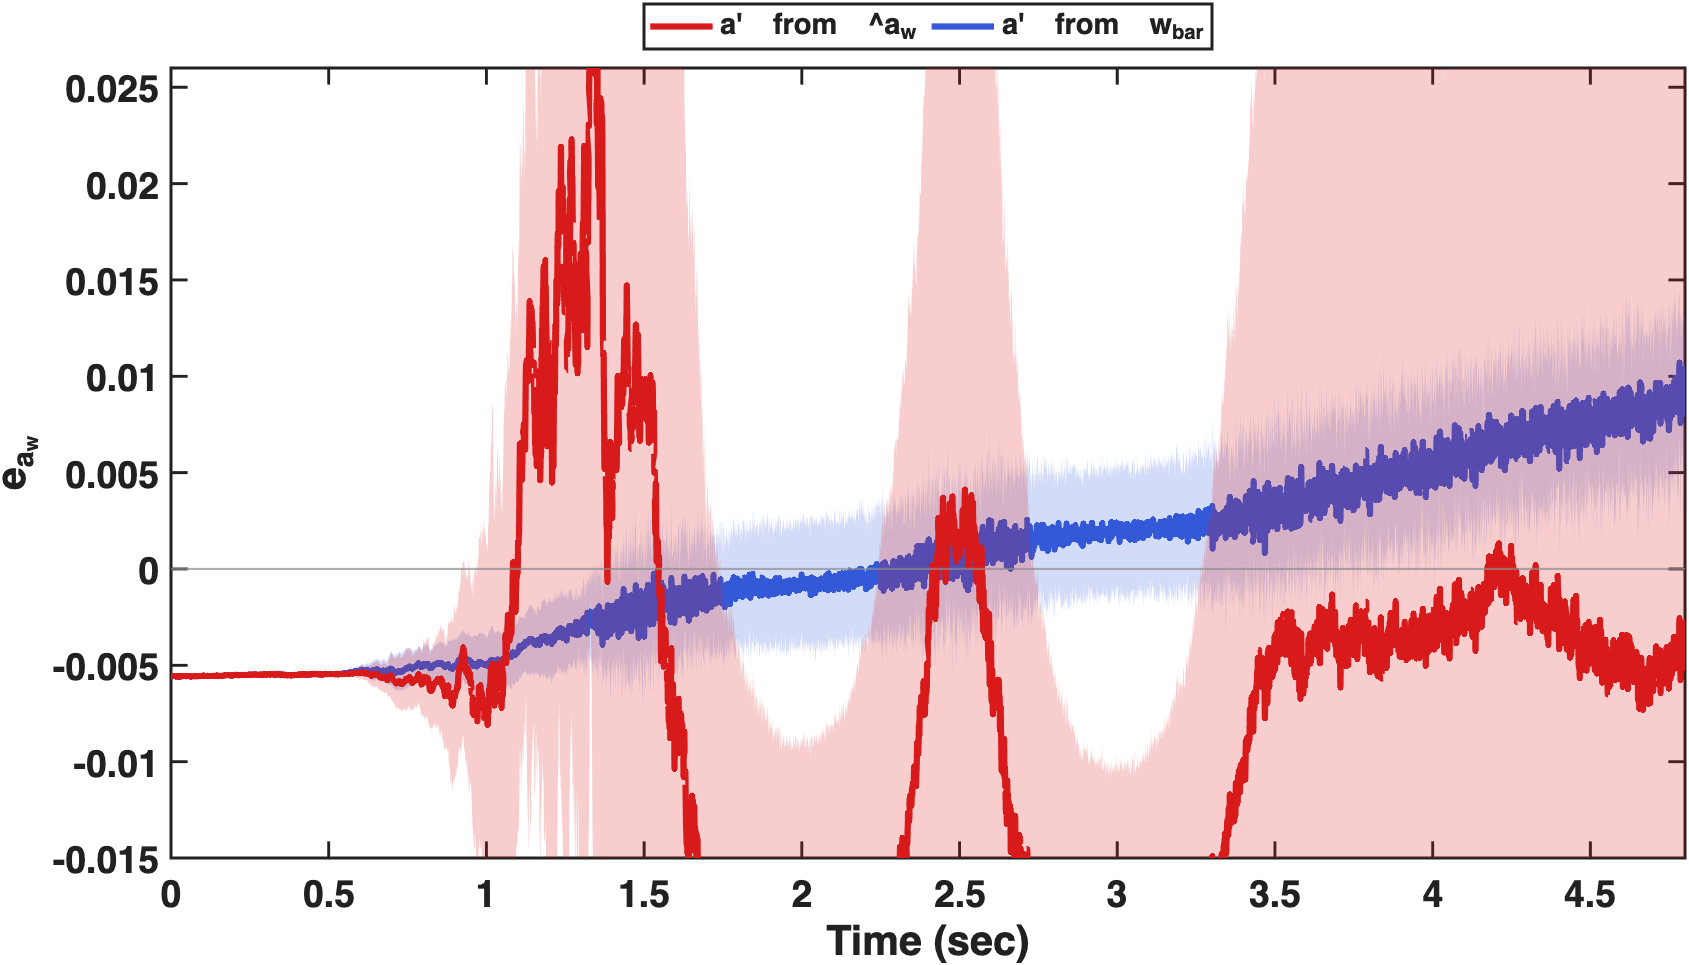
\includegraphics[width=\textwidth]{figures/formC_belief_vs_command.png}
\end{figure}

\begin{figure}[htbp]
\centering
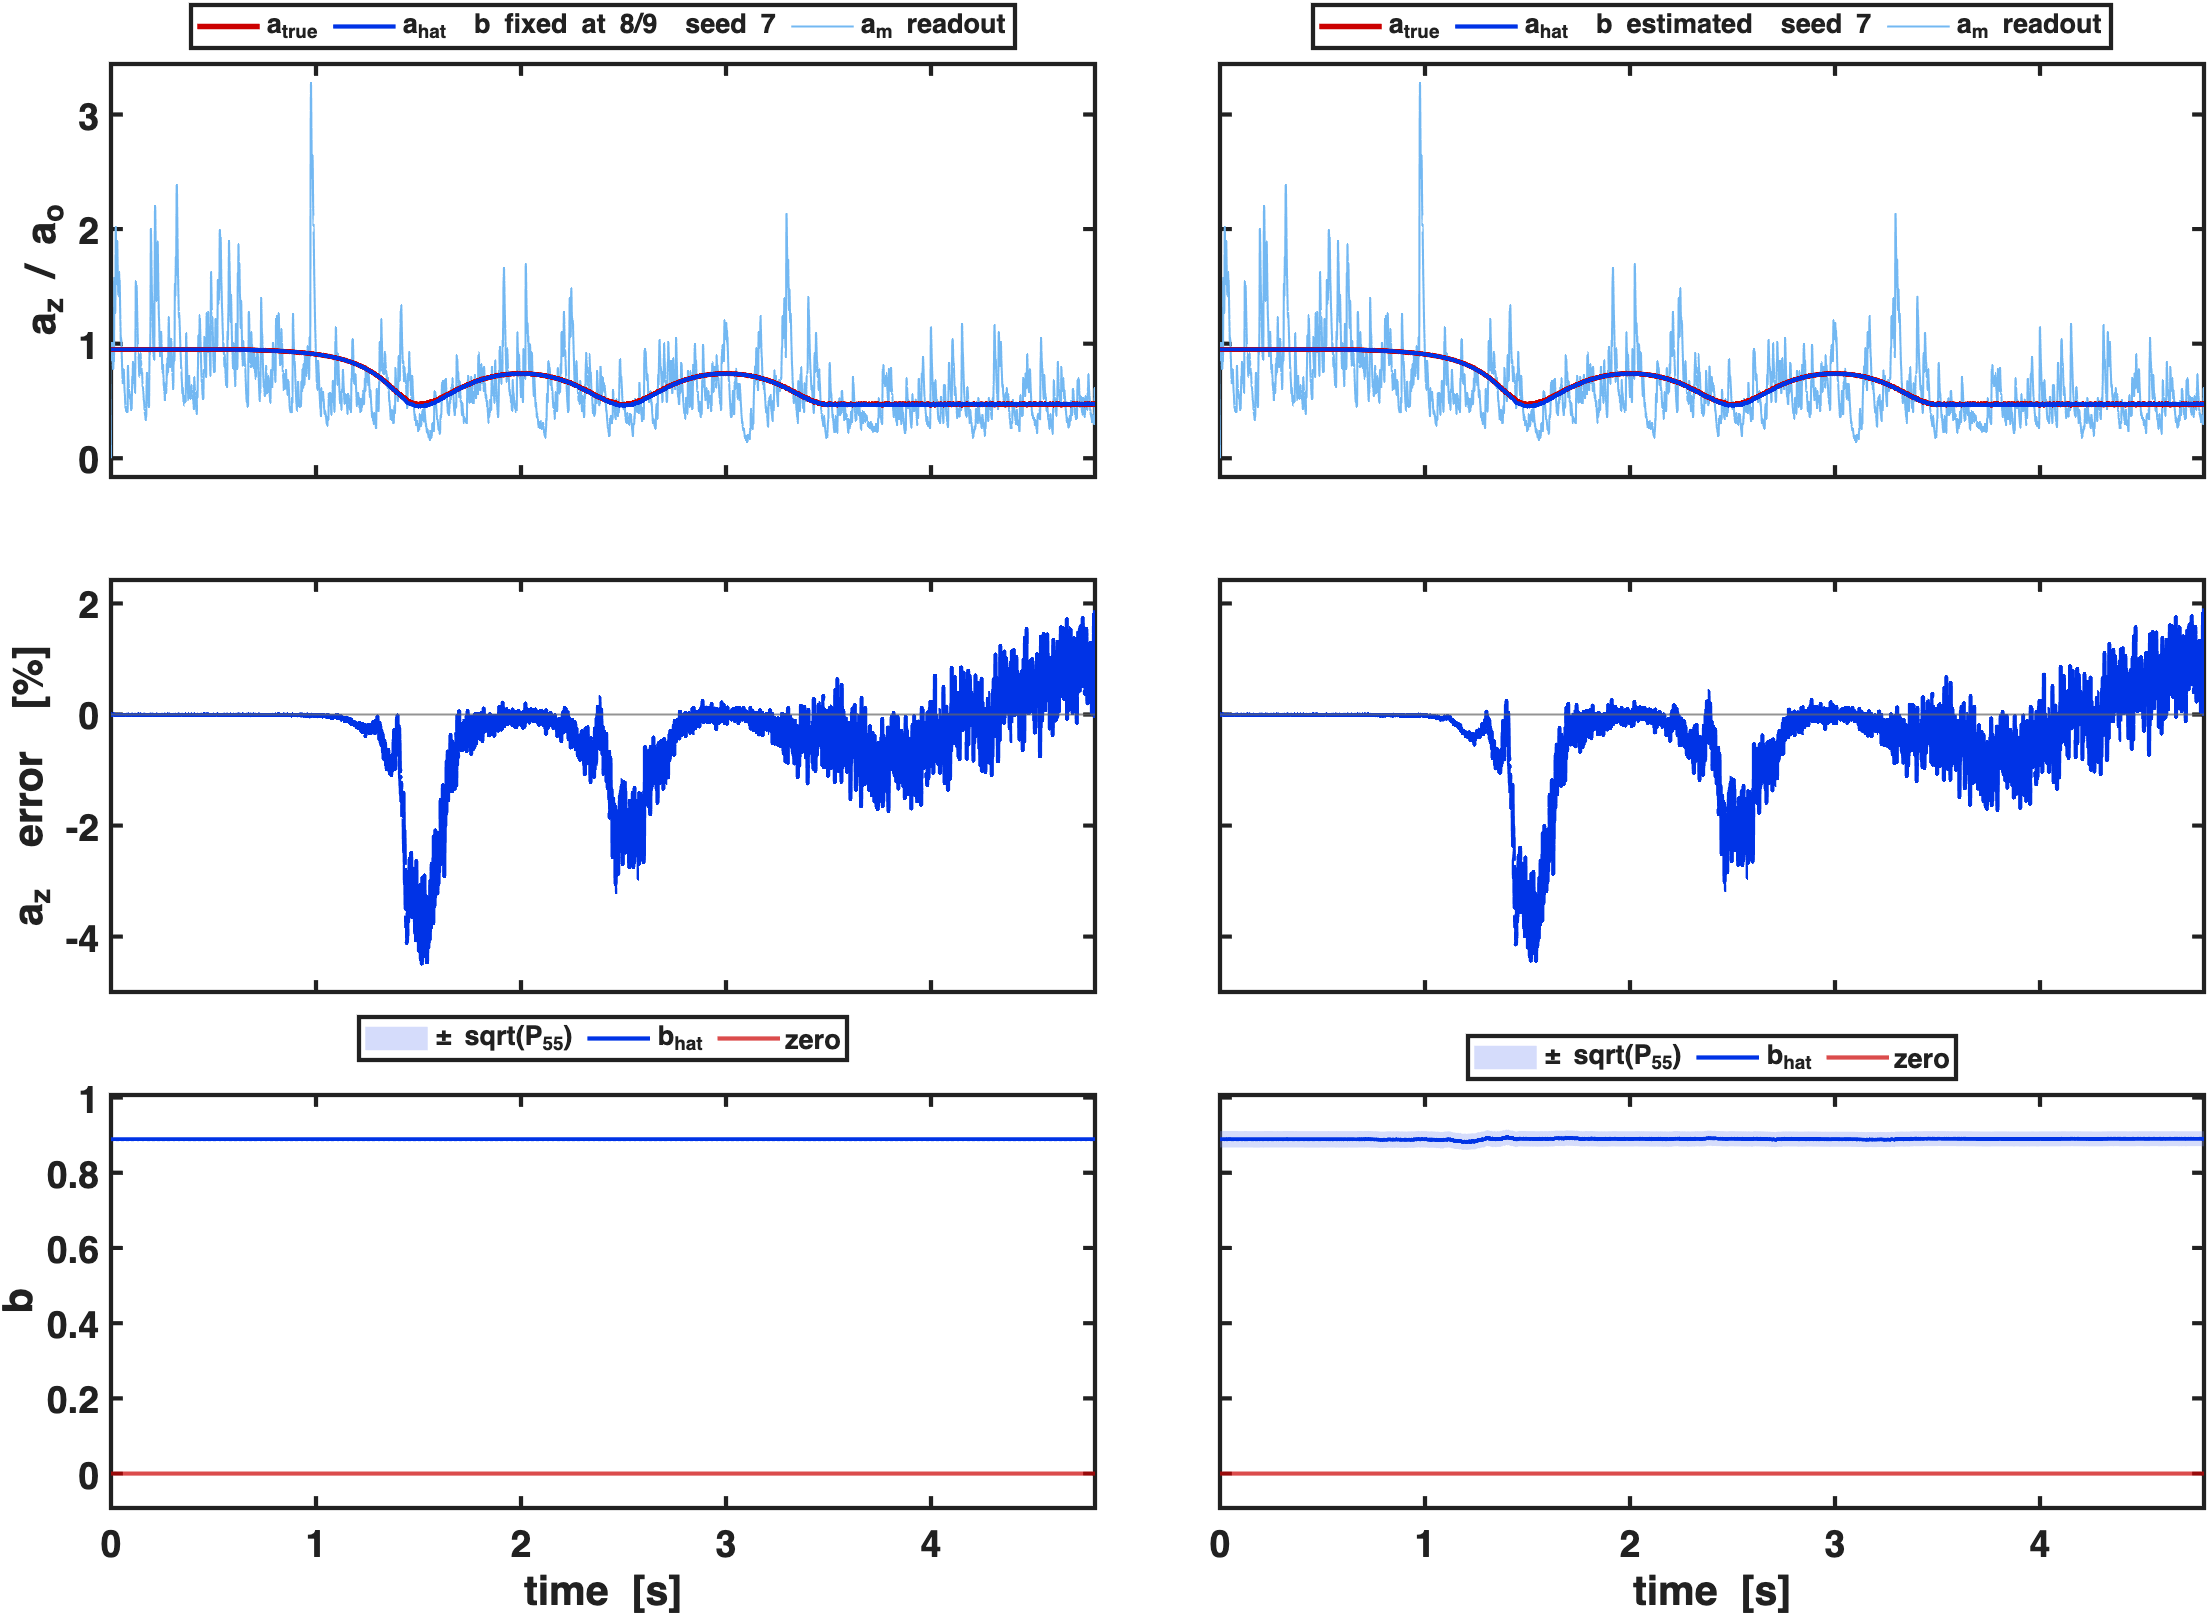
\includegraphics[width=\textwidth]{figures/formC_dist_cmp_xb_est_s07.png}
\end{figure}

\begin{figure}[htbp]
\centering
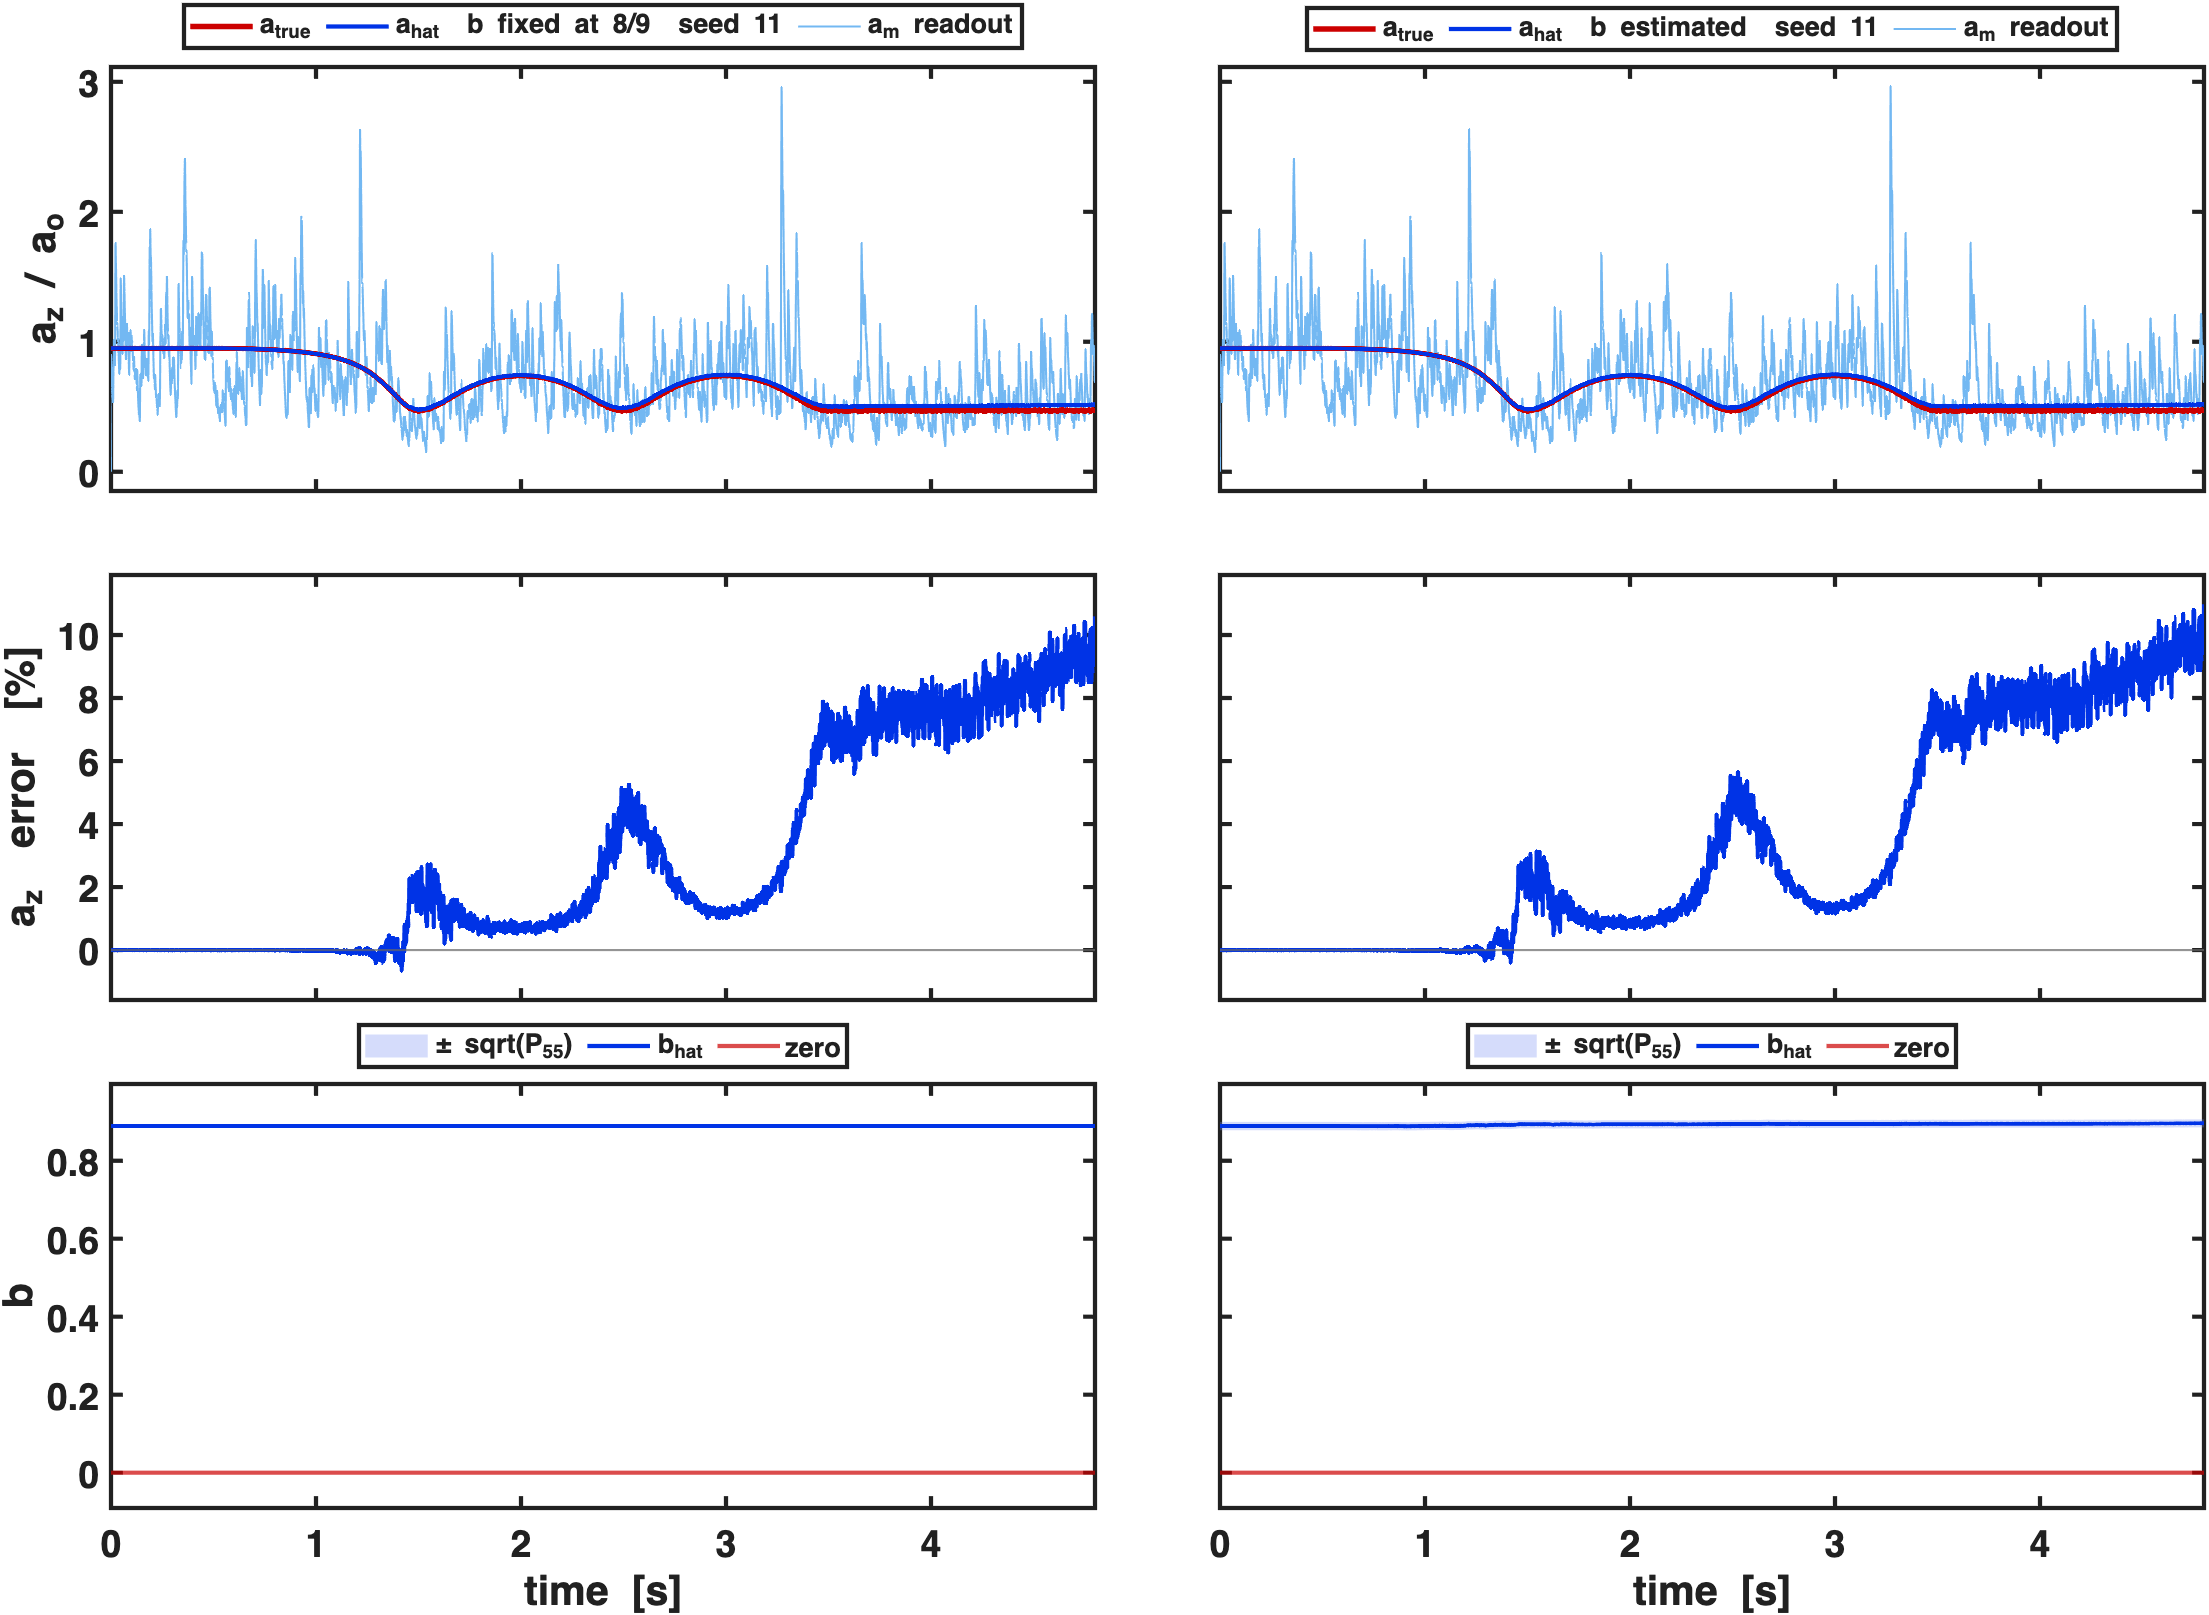
\includegraphics[width=\textwidth]{figures/formC_dist_cmp_xb_est_s11.png}
\end{figure}

\begin{figure}[htbp]
\centering
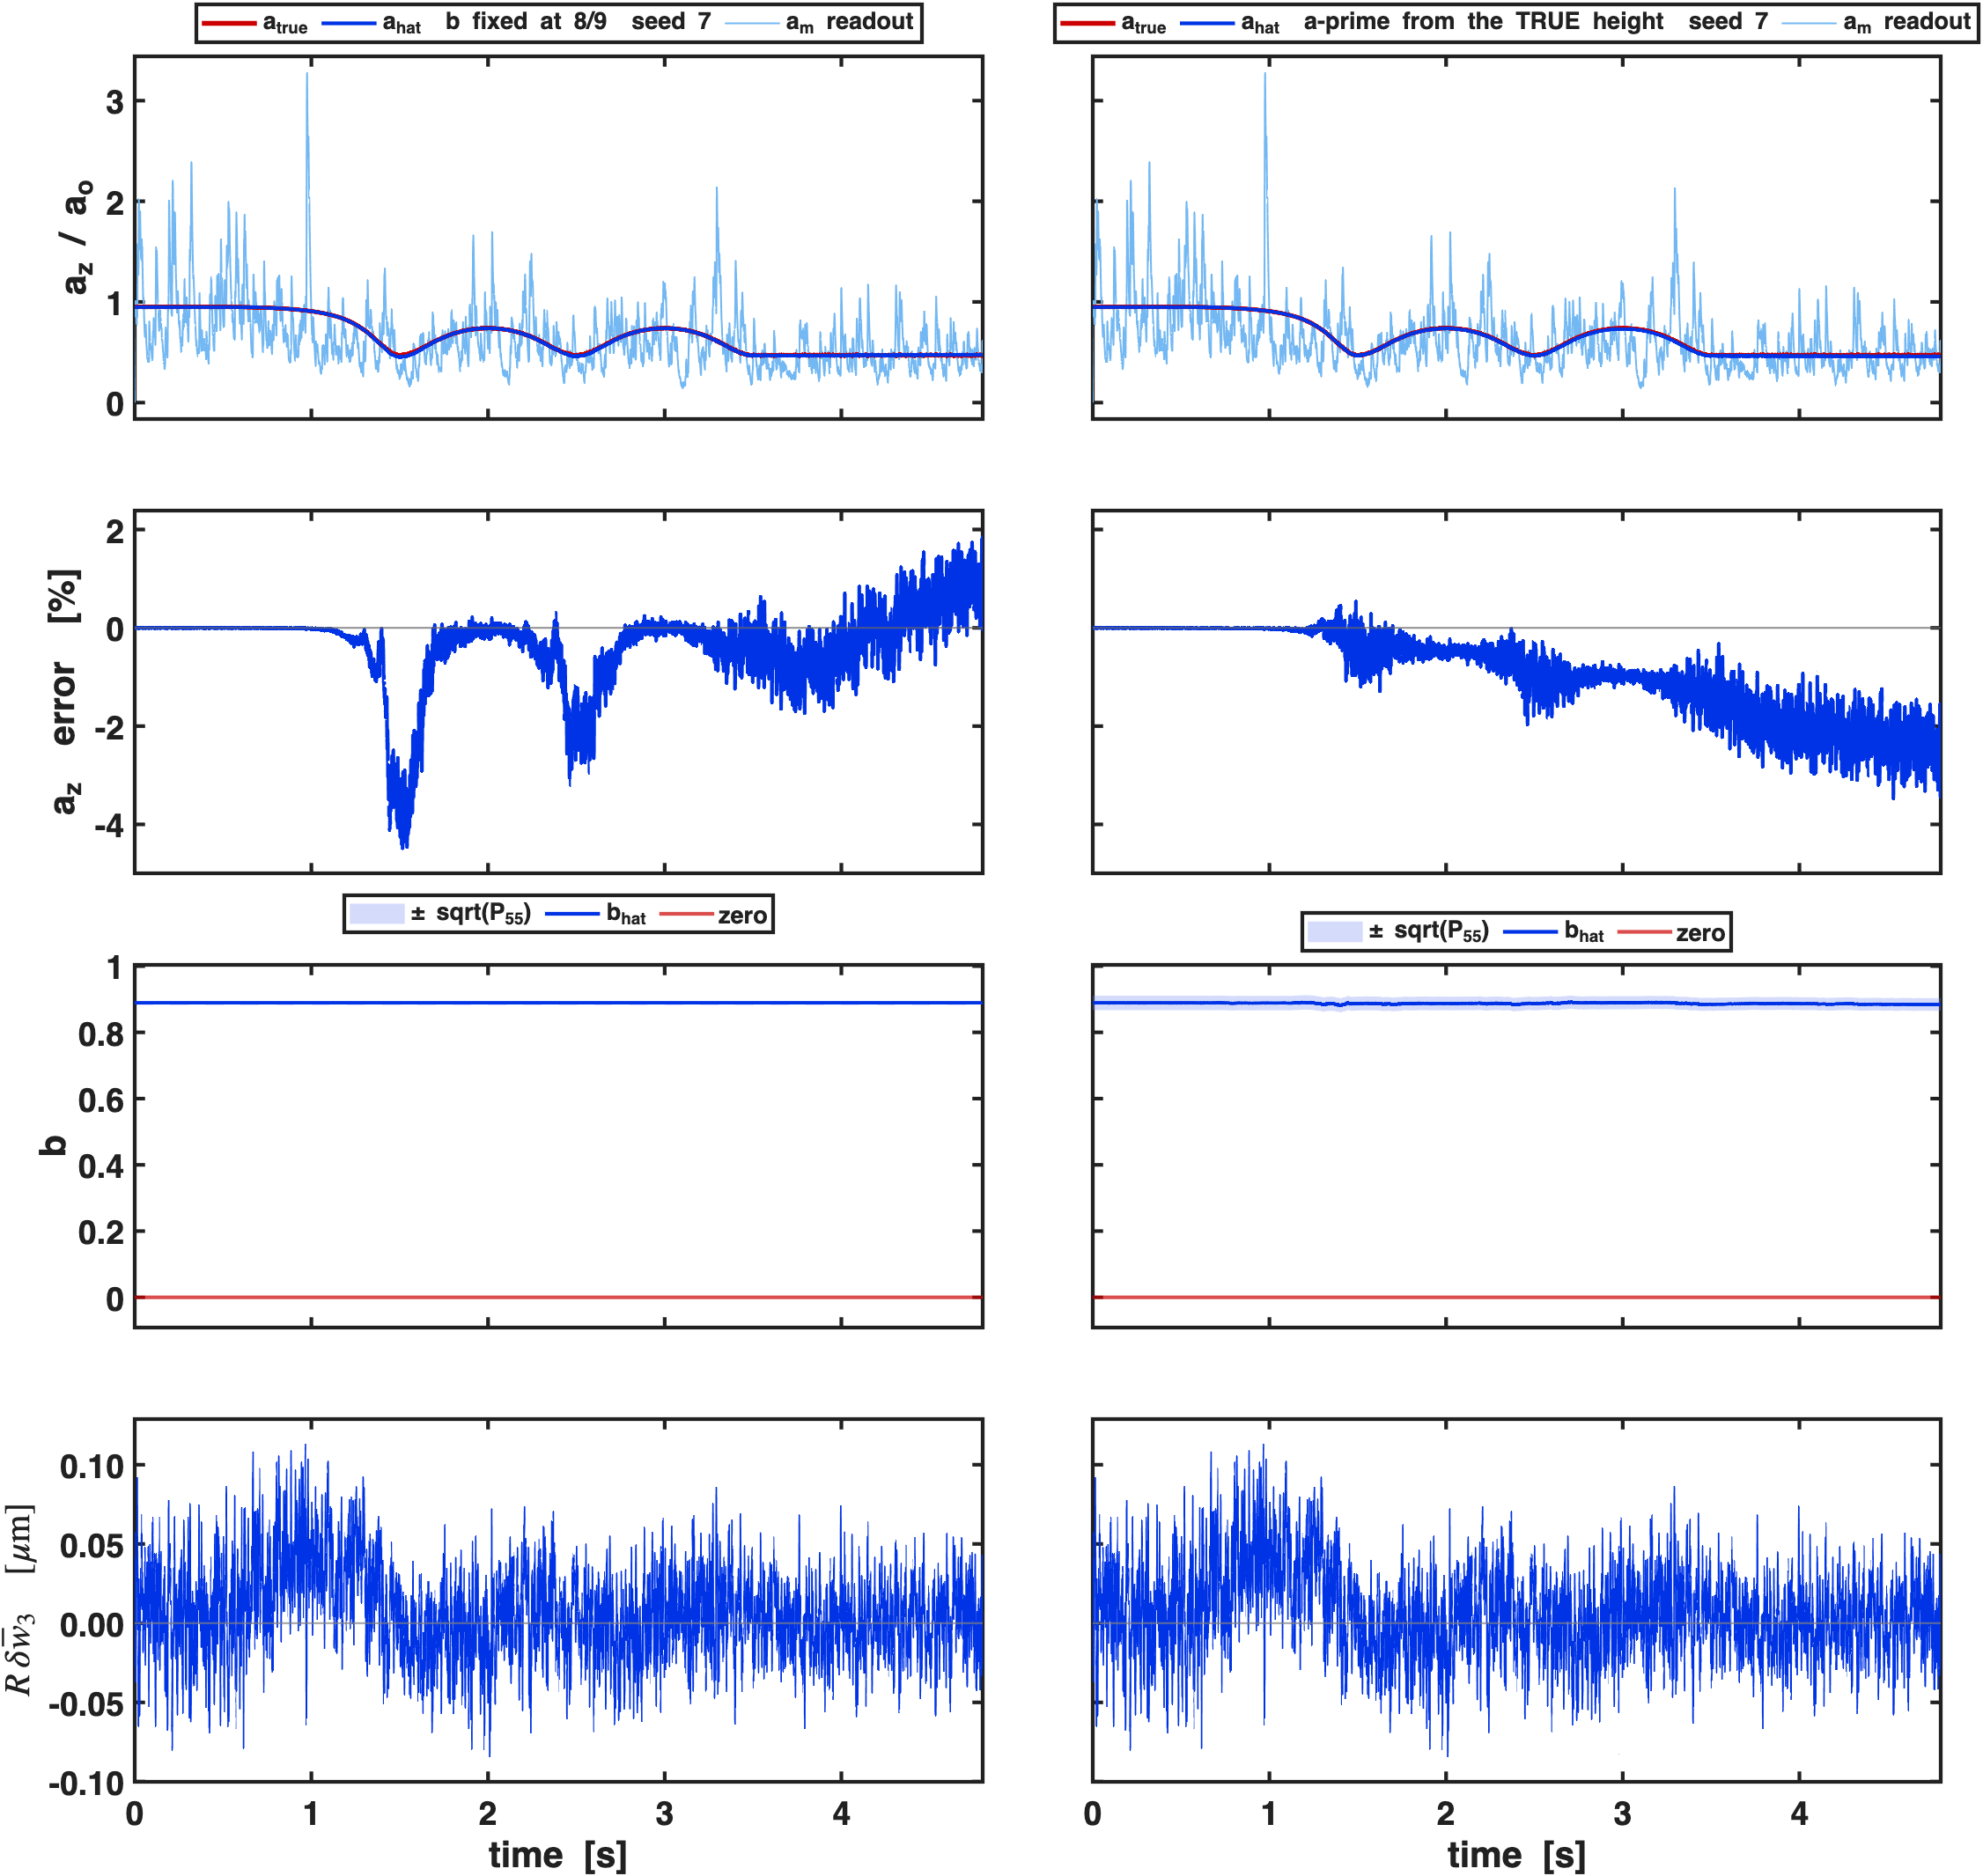
\includegraphics[width=\textwidth]{figures/formC_dist_cmp_xb_true_s07.png}
\end{figure}

\begin{figure}[htbp]
\centering
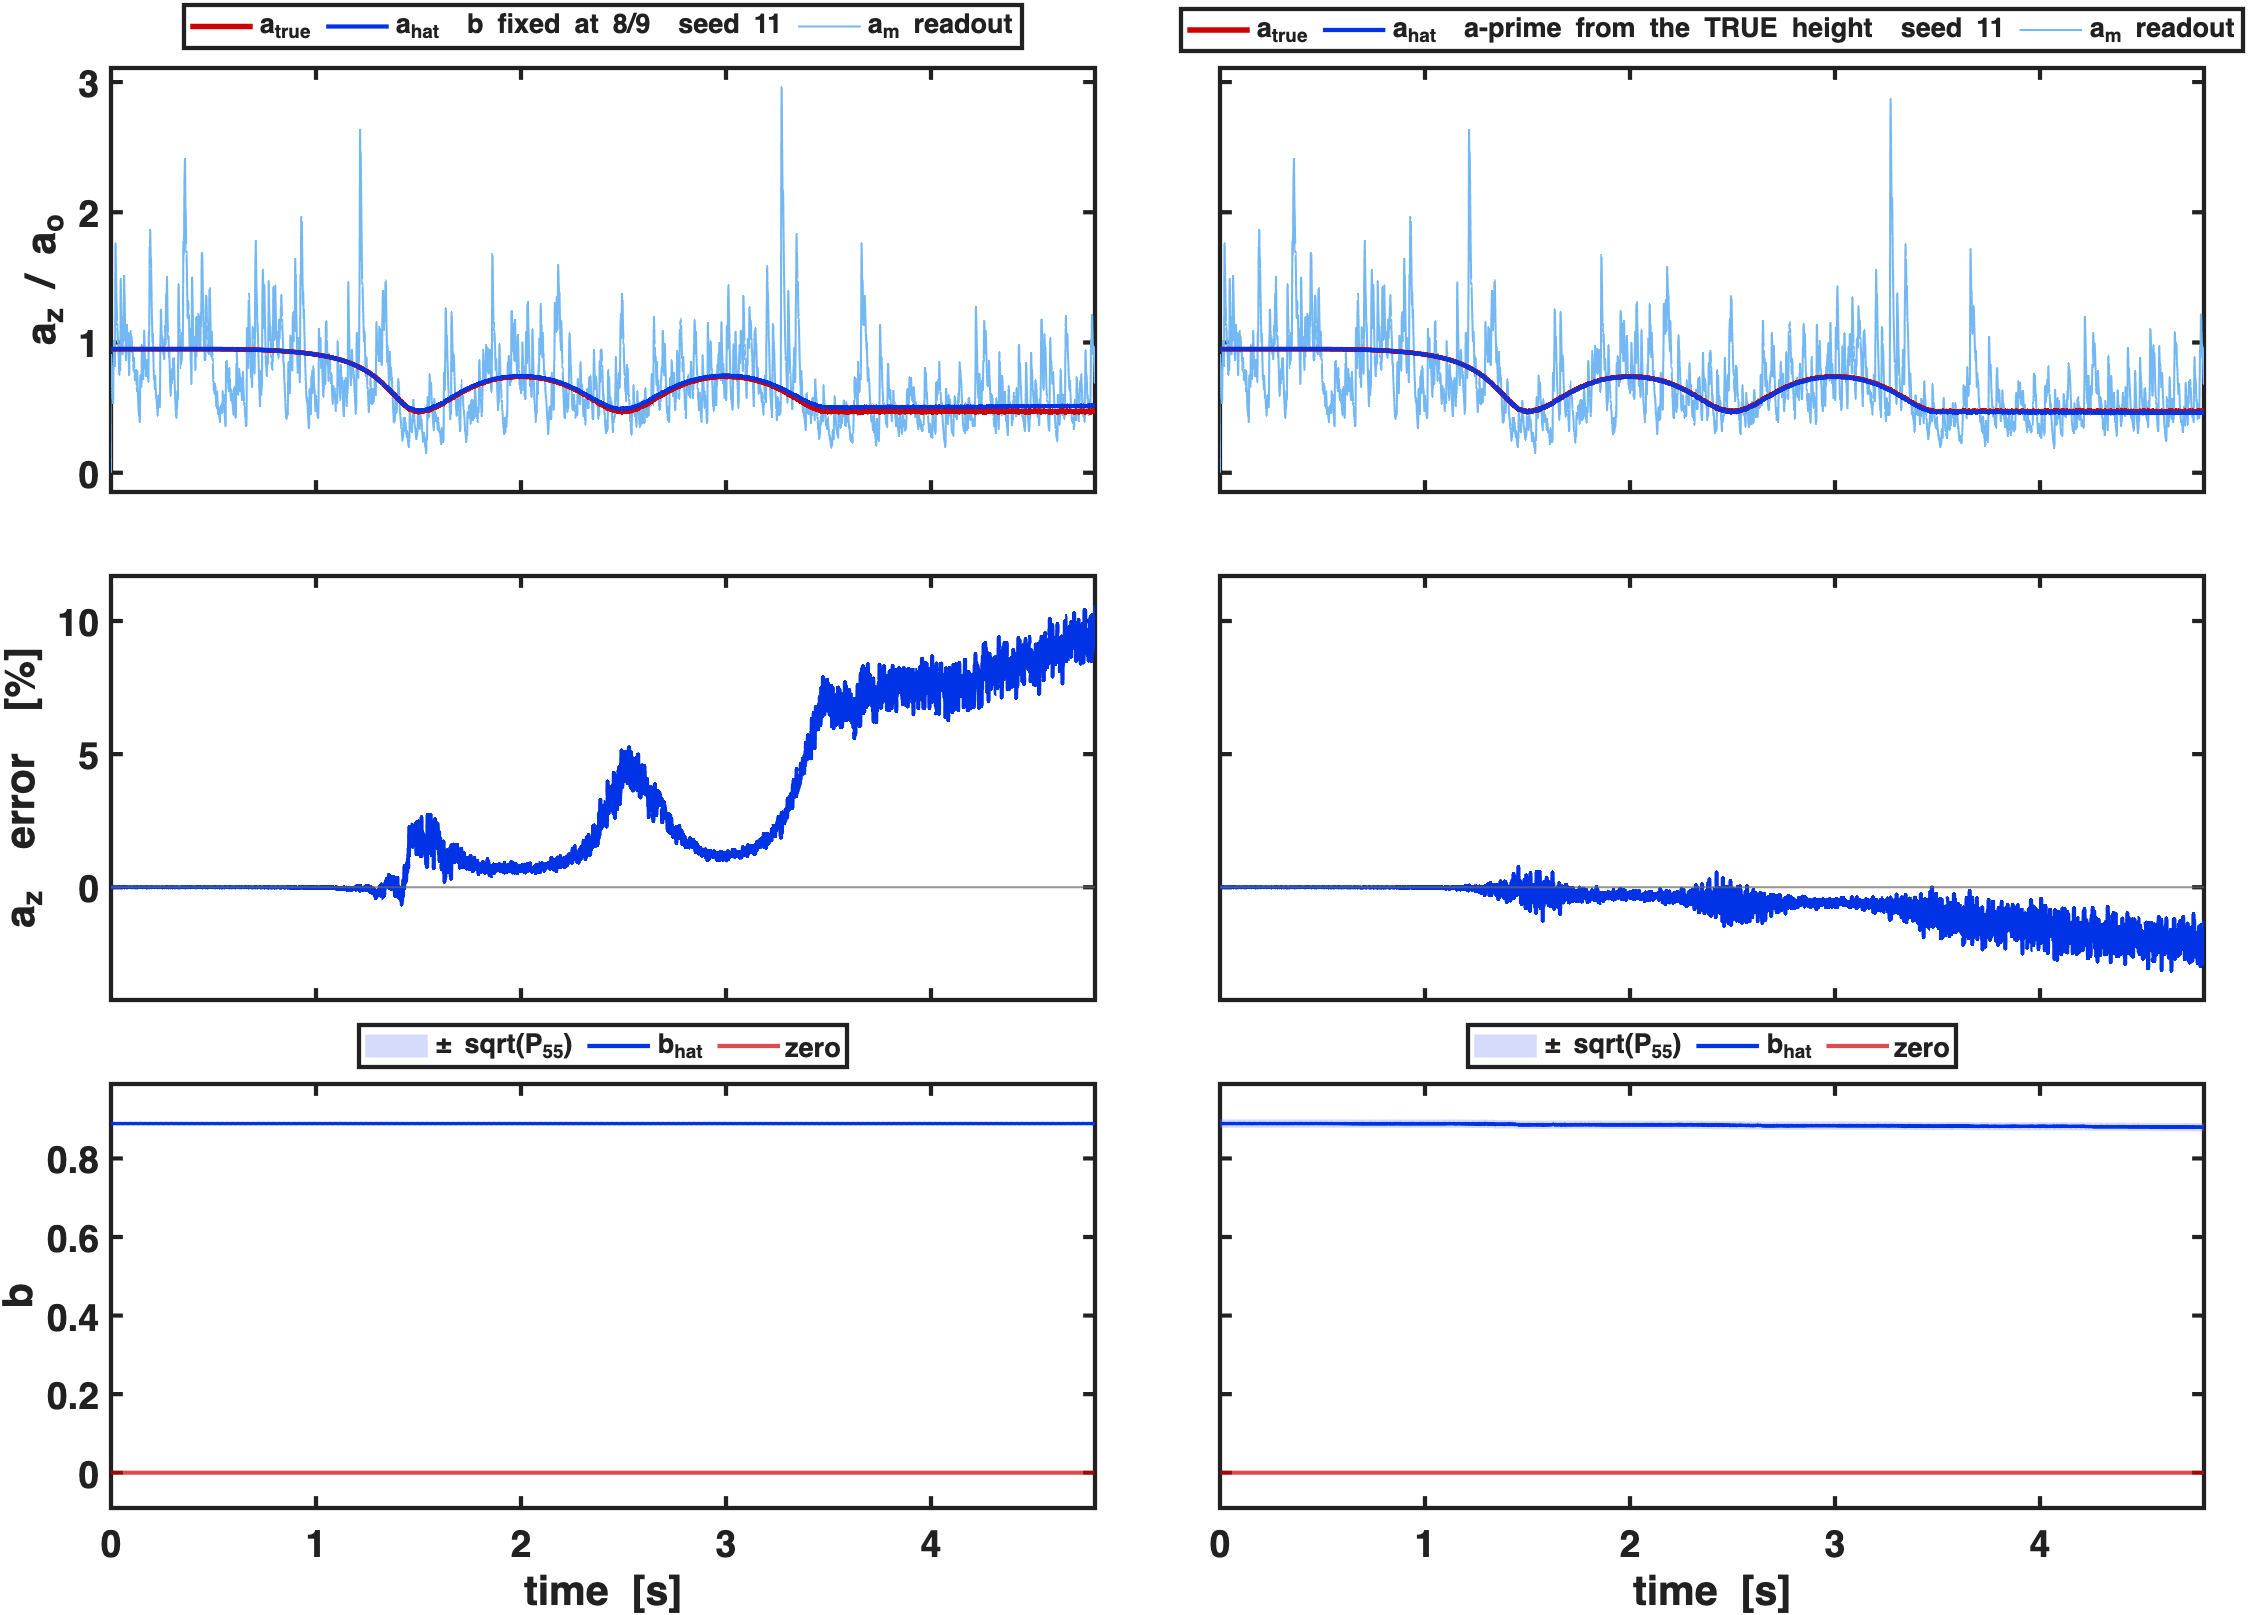
\includegraphics[width=\textwidth]{figures/formC_dist_cmp_xb_true_s11.png}
\end{figure}

\end{document}
